% This is samplepaper.tex, a sample chapter demonstrating the
% LLNCS macro package for Springer Computer Science proceedings;
% Version 2.20 of 2017/10/04
%
\documentclass[runningheads]{llncs}
%
\usepackage{graphicx}
% Used for displaying a sample figure. If possible, figure files should
% be included in EPS format.
%
% If you use the hyperref package, please uncomment the following line
% to display URLs in blue roman font according to Springer's eBook style:
% \renewcommand\UrlFont{\color{blue}\rmfamily}

\begin{document}
%
\title{A Study of Herbie effects on FPTaylor computation of error bounds \thanks{Supported by organization x.}}
%
%\titlerunning{Abbreviated paper title}
% If the paper title is too long for the running head, you can set
% an abbreviated paper title here
%
\author{Rocco Salvia, \and
Zvonimir Rakamari\'c}
%
\authorrunning{F. Author et al.}
% First names are abbreviated in the running head.
% If there are more than two authors, 'et al.' is used.
%
\institute{School of Computing, University of Utah, Salt Lake City UT 84112, USA \email{rocco@cs.utah.edu}\\ \email{zvonimir@cs.utah.edu}}
%
\maketitle              % typeset the header of the contribution
%
\begin{abstract}
Due to the variety of analyzers facing well known issues deriving from floating-point approximation errors, it is critical to find a way such that these tools can cooperate to better succeed in the analysis of approximate computing.
This work describes what the benefits of combining together FPTaylor and Herbie are on the same arithmetic expression. 
FPTaylor is a rigorous detector of approximation errors deriving from the quantization of real arithmetic into discrete arithmetic. FPTaylor detects and proves the maximum error produced by quantization for a bounded numeric interval.
Herbie is a rewriter tool, it rewrites the original expression to reduce the quantization error. Herbie produces a new expression with similar semantic with respect to the original one, but with a lower quantization error. The goal of this work is to empirically verify if Herbie rewrites result in a lower error bound in FPTaylor. On the other hand, we verify if FPTaylor may take advantage from Herbie and provides an alternative expression with respect to the original one. 

\keywords{First keyword  \and Second keyword \and Another keyword.}
\end{abstract}
%
%
%
\section{Introduction} Floating-point arithmetic makes real arithmetic feasible on computers, but it introduces approximation errors both in the conversion and during each computation. In real world, we need to bound to the approximation error introduced by floating-point arithmetic. For example, the use of coarse floating-point arithmetic can dramatically impact the results of some critical computations. In the past, there have been incidents caused by insufficient focus towards these approximation problems, which results in a waste of money and in the worst scenario in the loss of human lives.


The goal of verification is to compute an upper bound of the maximal approximation error a finite precision expression can generate. Given the inexact nature or the floating-point arithmetic, the main issue is that even small errors may affect the correct execution of a program.


There exist tools providing rigorous error bound estimation for an arithmetic expression together with a proof certificate to support such bound~\cite{fptaylor,magron,precisa,daisy}. FPTaylor~\cite{fptaylor} relies on symbolic Taylor expansions to quantify the error introduced by an arithmetic expression. Taylor expansions approximate the original expression with a summation of polynomials. In this way, the approximation error is kept as a symbolic coefficient of one of the terms in the summation.

Together with rigorous estimators, there exist floating-point analyzers looking for the best mixed-precision allocation for an expression or program. Their goal is to minimize the floating-point precision for an expression, e.g. whether the minimal configuration does not affect the accuracy of the result with respect to the original computation~\cite{mixedLam,herbgrind,precimonius}.
Unfortunately, these tools cannot test all possible configurations because of the huge space to scan (from 1 to 52 bits for each of the n variables in a program: it results in a space of $O(52^n)$, that can be drastically reduced to $O(3^n)$ if only half, single or double precision standards from IEEE 754~\cite{ieee} are used for the evaluation). 
The result is that heuristics are adopted, and only few configurations are tested without any rigorous guarantees.
Using a similar unsound approach, Herbie~\cite{herbie} is a tool that randomly scans the input domain of a formula and it detects sensitive input values producing high floating-point approximation errors. Herbie rewrites the expression to reduce the floating-point error in specific intervals of the domain. The result is that given an expression, Herbie may return multiple rewrites each one associated to a particular interval of the domain of the expression. Herbie aims to improve the accuracy of the expression for all input values.

Recent effort in floating-point tools combination results in a parallel project~\cite{daisyherbie} involving Daisy~\cite{daisy} and Herbie~\cite{herbie}. No matter the different tools adopted in the analysis, the main difference with this work concerns the approach used in the evaluation of the final product. In this work we use Herbie as an improvement to FPTaylor capabilities, e.g. as an additional power available in FPTaylor. Indeed our experiments compare FPTaylor against the combination FPTaylor with Herbie (FPTherbie). The motivation is mainly due to the different nature of these two analyzers. Herbie does not come with rigourous guarantee compared to the rigorous approach adopted by FPTaylor. In our intension, Herbie is a useful heuristic in addition to FPTaylor, and in this work we evaluate the accuracy of the rewriter.


The overview of this project is shown in Figure\ref{fig:architecture}. Given in input a floating-point expression and a bounded interval, FPTaylor returns the bound of the original expression (flow 1) together with the new bound on the rewritten expression (flow 2). 
Two goals are achieved from the new tool: (i) check how FPTaylor can benefit from Herbie in terms of number of reduced bounds and (ii) verify the reliability of Herbie in terms of $accuracy= \frac{lower bounds}{rewritten expressions}$
\begin{figure*}[t]
	\begin{center}
		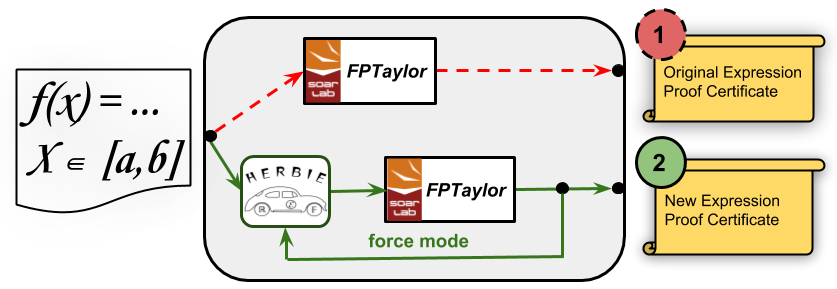
\includegraphics[width=\columnwidth]{picture}
	\end{center}
	\caption{Overview}\label{fig:architecture}
\end{figure*}

\section{Methodology}
In this work we evaluate our tool on all the benchmarks\footnote{Our benchmarks are available at https://github.com/soarlab/FPTaylord} reported in FPTaylor~\cite{fptaylor} repository. The main issue with Herbie benchmarks is that they do not come with a bounded interval for each variable in the expression.

First of all, the original expression is given as an input to FPTaylor which returns an upper bound for the approximation error generated by the expression. This flow corresponds to flow 1 in Figure.1.
In the second scenario (flow 2) (i) Herbie rewrites the expression and (ii) FPTaylor detects the new approximation bound.

Both Herbie and FPTaylor requires a dedicate format for input expressions. For this reason, this project relies on FPBench\footnote{https://github.com/FPBench/FPBench}, a repository containing formats converters among many floating-point analyzers. 
In particular, FPBench provides a converter from FPTaylor to Herbie format (and viceversa).

As described in Solovyev et al. FPTaylor does not currently support few functions (supported in Herbie) like the operator pow, and cbrt (cubic root). The way we patched this problem is asking Herbie to not use such functions when improving an expression (with the potential risk of missing the best improvement).

\section{Results}
\begin{table}
	\centering
	\caption{Experimental results for absolute round off errors.}\label{tab1}
	\begin{tabular}{|l|l|l|l|l|l|}
		\hline
		Name &  Or. Bound & New Bound & R.Fail. & Unk.Rew. &Ill.Rew.\\
		\hline
		sine & 4.43e-16& FAILURE& 0& 0& 3(/0)\\
		sineOrder3 & 5.93e-16& 5.93e-16& 0& 0& 0\\
		sqroot & 5.01e-16& FAILURE& 0& 20& 0\\
		t\_div\_t1 & 2.21e-16 & 2.21e-16 & 0& 0& 0\\
		carbonGas & 5.90046e-09 & 5.900398e-09& 0& 0& 0\\
		doppler1 & 1.21e-13 & 1.21e-13& 2& 0& 0\\
		doppler2 & 2.22e-13 & 2.22e-13 & 2& 1& 1(/0)\\
		doppler3 & 6.62e-14 & 6.62e-14 & 2& 0& 0\\
		himmilbeau & 1.10e-12 & 1.10e-12 & 0& 0& 0\\
		jetEngine & 1.03e-11 & 1.03e-11 & 0& 0& 0\\
		kepler0 & 7.46e-14 & 7.46e-14 & 0& 0& 0\\
		kepler1 & 2.86e-13 & 2.86e-13 & 0& 0& 1(/0)\\
		kepler2 & 1.57e-12 & 1.57e-12 & 0& 0& 0\\
		predPrey & 1.58e-16 & 1.55e-16 & 2& 10& 0\\
		rigidBody1 & 2.94e-13 & 2.77e-13 & 0& 0& 0\\
		rigidBody2 & 3.60e-11 & 3.38e-11 & 0& 0& 0\\
		turbine1 & 1.66e-14 & 1.66e-14 & 2& 0& 0\\
		turbine2 & 2.00e-14 & 2.00e-14 & 3& 0& 0\\
		turbine3 & 9.57e-15& FAILURE& 0& 0& 3(+$\infty$)\\
		verhulst & 2.47e-16 & 2.41e-16 & 6& 2& 0\\
		azimuth & 8 .90e-15 & 5.11e-15 & 0& 0& 0\\
		hartman & 4.60e-15 & 3.48e-15& 2& 0& 0\\
		logexp & 1.98e-15& 1.49e-15& 0& 1& 0\\
		sphere & 8.10e-15& 7.49e-15& 0& 0& 0\\
		TOT & / & / & 21 & 34 &8\\		
		\hline
	\end{tabular}
\end{table}
Table.1 reports the evaluation of all the benchmarks in~\cite{fptaylor}. The columns Name shows the name of the expression. Or.Bound is the bound of the expression reported in[1], while New Bound is the new bound proved by FPTaylor on the rewritten expression. Rewrite Failures counts how many times Herbie rewrites the expression but FPTaylor proves a larger bound with respect to the original one.
Unknown Rewrites reports how many times Herbie provides new expressions containing functions not yet implemented in FPTaylor (pow, cbrt, etc.). Illegal Rewrites column reports how many times the rewritten expression contains a potential bug (detected by FPTaylor analysis). It means, FPTaylor detects the new expression may result in a division by zero in the given interval. All of these Illegal Rewrites were manually verified in the expression and they are all true positive bugs.
Out of the 24 benchmarks, for $\frac{21}{24}$ benchmarks Herbie provides an expression with a bound at least equal to the original one. While for $\frac{9}{24}$ benchmarks Herbie strictly reduces the final error bound of the expression. 
Given the 21 positive results Herbie needs in average one failing rewrite before improving the expression (a true improvement is when FPTaylor proves newBound<=origBound).
For $\frac{3}{24}$ benchmarks the rewrite does not produce a valid expression. In both sine and turbine3 all the rewrites contains a bug (with a division by zero expression). 
In case of sqroot all the rewrites from Herbie contain operators unsupported in FPTaylor.

\section{Discussion}
This project presents a new tool resulting from the combination of Herbie~\cite{herbie} and FPTaylor~\cite{fptaylor}. 
Herbie aims to improve the accuracy of an expression globally for the all domain of the function. It randomly samples the given expression and it identifies where the function suffers the most from approximation error. 
The main problem with Herbie is that profiling might not be accurate enough, resulting in a partial improvement of the function in some intervals, while it degrades the accuracy for others. Due to the unsoundness of the tool, the rewritten expression might not actually reduce the error bound of the original expression and FPTaylor may detect a loss with respect to the original bound. FPTaylor is a rigorous estimator of the approximation error of a function in a given interval.
The results shown how Herbie does not work well on FPTaylor benchmarks. Out of the 24 benchmarks only in $\frac{9}{24}$ Herbie improves the original expression, while in half the benchmarks Herbie provides a false positive to FPTaylor.
A future works might be the not trivial task of manually modify Herbie benchmarks and provide a bounded interval for each variable in the expression. 
It might be that FPTaylor benchmarks are already optimized. Indeed, the challenge for rigorous estimators (FPTaylor~\cite{fptaylor}, Daisy~\cite{Daisy}, PRECISA~\cite{precisa}, etc.) is to provide a least upper bound to the true unknown error of a given expression. Probably FPTaylor benchmarks are already optimized to make the job hard to estimators looking for a minimal error bound.

% ---- Bibliography ----
%
% BibTeX users should specify bibliography style 'splncs04'.
% References will then be sorted and formatted in the correct style.
%
\bibliographystyle{splncs04}
\bibliography{bibfile}
\end{document}
\grid
\grid
\grid
